\documentclass[11pt]{article}
\usepackage[a4paper,margin=1in]{geometry}
\usepackage{amsmath,amssymb}
\usepackage{booktabs}
\usepackage{graphicx}
\usepackage{hyperref}
\usepackage{tikz}
\usepackage{pgfplots}
\pgfplotsset{compat=1.18}
\usepackage{tikz}
\title{Deterministic Causal Boolean Integration: Short Rules for Complex Behaviour}
\author{Alberto Hern\'andez}
\date{}

\begin{document}
\maketitle

\begin{abstract}
We present a mechanism-first deterministic programme for causal Boolean networks that reconstructs global behaviours from exact, closed-form per-node rules. In contrast to probabilistic generative approaches, we emphasise concise causal mechanisms and ordering-aware index sets that yield complete repertoire equality under unbiased inputs. The programme delivers canonical structural representations, invariance under bit-order transforms, rigorous tests, reproducible artefacts, and professionally compiled documentation. Building on the broader argument that causal generative models more faithfully capture structure in complex systems, we demonstrate that short rules can create richly complex behaviours while retaining deterministic verifiability.
\end{abstract}

\section{Introduction}
Complex behaviours often admit simple causal generators. Our approach adopts a deterministic, Newton--Einstein style paradigm: discover minimal rules that explain maximal structure. We operate on Boolean networks with ordered inputs and exact per-node index-set formulae, composing columns to reconstruct outputs. This yields equality with exhaustive maps while enabling rigorous analysis and reproducibility.

Historically, information integration frameworks motivated sensitivity and structural measures but suffered from probabilistic ambiguities. Here we abandon integration and pursue fully deterministic causal reconstruction. The manuscript consolidates algorithms and experiments compiled in \texttt{expProcess.tex}, with ordering conventions, canonical programmes, and tests.

\section{Related Work}
Algorithmic generative models advocate causal mechanisms over purely probabilistic descriptions. Foundational works in causality, information theory, partial information decomposition, transfer entropy, and multi-information have clarified the axes along which deterministic rules can be assessed: causality (Pearl), information transfer (Schreiber), decomposition of joint effects (Williams--Beer; Lizier \emph{et al}.), and multi-source structure (Watanabe). Algorithmic information theory and complexity (Li--Vit\'anyi; Bennett \emph{et al}.) frame the succinctness of rules.

\section{Framework}
Inputs are enumerated deterministically with ordering policy and an explicit bit-reversal mapping $\varphi$. Per-node closed-form index sets are evaluated over ordered inputs; columns are composed to reconstruct full outputs. Canonical programmes consist of triplets $\langle\text{gate}, I_c, \theta\rangle$ per node and are invariant under node permutation modulo column order. Deterministic seeds and parameters ensure identical runs produce identical artefacts.

\section{Theory}
\subsection{Axioms}
\textbf{Axiom 1 (Ordering Invariance).} Let inputs be ordered either LSB-first or MSB-first. Define $\varphi:\{1,\dots,2^n\}\to\{1,\dots,2^n\}$ by $\varphi(j)=1+\mathrm{binrev}_n(j-1)$. For all networks and per-node programmes $\langle\text{gate}, I_c, \theta\rangle$, the one-step map satisfies $F_{\mathrm{MSB}}(j)=F_{\mathrm{LSB}}(\varphi(j))$.\\
\textbf{Axiom 2 (Canonical Composition).} For each node $i$, the output is $y_i=g_i\big(x_{I_c(i)};\theta_i\big)$, where $g_i$ acts on the subvector indexed by $I_c(i)$. The global map is the column-wise composition $F(x)=\big(y_1,\dots,y_n\big)$, invariant under node relabelling up to column permutation.\\
\textbf{Axiom 3 (Closure and Compositionality).} Index-set operations (union, intersection, complement) evaluated over ordered inputs preserve equality to gate evaluations; composing per-node columns reconstructs the global outputs exactly.\\
\textbf{Axiom 4 (Block Factorisation).} If the undirected adjacency $A=\mathbb{1}[cm+cm^\top>0]$ decomposes into disjoint blocks $\{B_k\}$ with no inter-block edges, then any additive compression functional $\mathcal{C}$ on the one-step map factorises: $\mathcal{C}(cm,\mathrm{dynamic})=\sum_k \mathcal{C}\big(cm[B_k,B_k],\mathrm{dynamic}[B_k]\big)$.

\subsection{Theorems and Proofs}
\textbf{Theorem 1 (Predictive Equals Baseline).} For all inputs $x\in\{0,1\}^n$, the predictive evaluation $F(x)$ equals the baseline dispatch $F_{\mathrm{TT}}(x)$ that uses per-node truth-table lookup.\\
\emph{Proof.} For any node $i$, the truth table $T_i$ encodes $g_i$ on $x_{I_c(i)}$. The predictive evaluation substitutes $x_{I_c(i)}$ directly into $g_i$, while the baseline returns $T_i\big(x_{I_c(i)}\big)$. Hence $y_i= T_i\big(x_{I_c(i)}\big)$ for all $i$, and column composition yields $F=F_{\mathrm{TT}}$.\\
\textbf{Theorem 2 (Ordering Invariance under $\varphi$).} With $\varphi$ as in Axiom 1, $F_{\mathrm{MSB}}(j)=F_{\mathrm{LSB}}(\varphi(j))$ for all $j$.\\
\emph{Proof.} $\mathrm{binrev}_n$ reverses the bit order of index codes, so $x^{\mathrm{MSB}}(j)=\mathrm{Reverse}\big(x^{\mathrm{LSB}}(\varphi(j))\big)$. Gate semantics depend only on the values of selected inputs, not on enumeration order; thus per-node outputs match after remapping row indices, and columns compose to give the stated equality.\\
\textbf{Theorem 3 (Block Factorisation).} Under the hypothesis of Axiom 4, the one-step map decomposes into independent submaps $F(x)=\big(F_{B_1}(x_{B_1}),\dots,F_{B_m}(x_{B_m})\big)$, and any additive $\mathcal{C}$ satisfies $\mathcal{C}(F)=\sum_k \mathcal{C}(F_{B_k})$.\\
\emph{Proof.} With no inter-block edges, each $y_i$ depends only on inputs within its block. Therefore $F$ is a Cartesian product of submaps. Additivity yields the stated factorisation.\\
\textbf{Theorem 4 (Exact Gate Robustness under Bit-Flips).} Let $z\in\{0,1\}^k$ be i.i.d. flips with rate $q$ and $\rho=1-2q$. For parity gates of arity $k$, $\Pr\big[g(x)=g(x\oplus z)\big]=\tfrac{1+\rho^k}{2}$. For monotone gates, first-order decay is governed by total influence $\mathrm{Inf}(g)$: $\Pr[\text{error}]\approx \mathrm{Inf}(g)\,q$ as $q\to 0$.\\
\emph{Proof.} For parity, correctness requires an even number of flips; the even-flip probability is $(1+\rho^k)/2$. Influence expansion gives the monotone first-order term.\\
\textbf{Theorem 5 (Information Signatures for Deterministic Gates).} Under unbiased inputs: XOR/XNOR have $I(x_i;y)=0$, $I(x_1,x_2;y)=1$, PID synergy $=1$, redundancy $=\mathrm{Unique}_i=0$; transfer entropy $TE_{X\to Y}=TE_{Y\to Y}=1$, total correlation $TC=1$. AND/OR/NAND/NOR have $I(x_i;y)=\log_2\tfrac{4}{3}\approx 0.311$, $I(x_1,x_2;y)\approx 0.811$, modest positive synergy, $TE_{X\to Y}=TE_{Y\to Y}=\tfrac{1}{2}$, and $TC\approx 0.811$.\\
\emph{Proof.} Build exact joint distributions from truth tables; compute mutual informations and conditional informations. For deterministic maps, $TC=H(y)$; XOR has $H(y)=1$, monotone gates have $H(y)=H(\mathrm{Bernoulli}(\tfrac{3}{4}))\approx 0.811$. PID components follow from $I_{\min}$ redundancy and the identities $I=\mathrm{red}+\mathrm{uniq}+\mathrm{syn}$. Transfer entropy reduces to conditional mutual information under the stated update.

\section{Methods and Validation}
Baseline exhaustive one-step maps are compared against predictive analytic reconstructions. Ordering-aware tests verify invariance under $\varphi$. Artefacts are exported as JSON and \LaTeX tables; documentation is compiled in British English. Ensembles and heuristics include ER, scale-free, and small-world constructions, subsystem searches via connected components, and noise robustness assays for gates and networks.

\subsection{Deterministic Evaluation and Ordering}
Inputs are enumerated deterministically; LSB/MSB orderings are related by the involution $\varphi$. Per-node evaluation applies $g_i$ to $x_{I_c(i)}$; columns compose to $F(x)$. Canonical triplets $\langle\text{gate}, I_c, \theta\rangle$ define the programme; ordering invariance ensures repertoire equality modulo $\varphi$.

\subsection{Algorithmic Procedures}
\textbf{Algorithm: Deterministic Per-Row Predictive Evaluation}\\
\begin{center}
\begin{tabular}{rl}
\hline
Step & Description \\
\hline
1 & Input: connectivity $cm$, per-node $\langle\text{gate}, I_c, \theta\rangle$, ordering policy \\
2 & Enumerate inputs $x\in\{0,1\}^n$ deterministically (LSB or MSB) \\
3 & For each node $i$, compute $y_i=g_i\big(x_{I_c(i)};\theta_i\big)$ \\
4 & Compose columns to form $F(x)=\big(y_1,\dots,y_n\big)$ \\
5 & Repeat for all $x$ (or sampled rows) and record artefacts \\
6 & Output: repertoire $F$, timings, memory; ordering invariance via $\varphi$ \\
\hline
\end{tabular}
\end{center}

\textbf{Algorithm: Importance Sampling Equality at Large $n$}\\
\begin{center}
\begin{tabular}{rl}
\hline
Step & Description \\
\hline
1 & Input: $cm$, programme $\langle\text{gate}, I_c, \theta\rangle$, sample size $m$ \\
2 & Partition by Hamming strata $\{w=0,1,\lfloor n/2\rfloor,n-1,n\}$ \\
3 & Draw $m$ rows across strata deterministically (fixed seeds) \\
4 & Compute predictive $F(x)$ per row by per-node evaluation \\
5 & Compute baseline $F_{\mathrm{TT}}(x)$ by truth-table lookup \\
6 & Verify $F(x)=F_{\mathrm{TT}}(x)$; export accuracy, timings, memory \\
\hline
\end{tabular}
\end{center}

\textbf{Algorithm: Subsystem Blocks via Connected Components}\\
\begin{center}
\begin{tabular}{rl}
\hline
Step & Description \\
\hline
1 & Input: $cm\in\{0,1\}^{n\times n}$, zero diagonal \\
2 & Build undirected adjacency $A=\mathbb{1}[cm+cm^\top>0]$ \\
3 & Compute connected components of $A$ to obtain blocks $\{B_k\}$ \\
4 & Compute cut fraction $\phi=E_{\mathrm{cut}}/E$ and $\Delta\mathcal{C}$ \\
5 & Accept factorisation when $\phi=0$ and $\Delta\mathcal{C}=0$ \\
6 & Output: blocks, metrics, artefacts (Blocks.tex, Status.txt) \\
\hline
\end{tabular}
\end{center}

\textbf{Algorithm: Gate-Level Noise Robustness (Exact)}\\
\begin{center}
\begin{tabular}{rl}
\hline
Step & Description \\
\hline
1 & Input: gate $g$, arity $k$, flip rate $q$ \\
2 & Enumerate inputs $x\in\{0,1\}^k$ and noise masks $z\in\{0,1\}^k$ \\
3 & Compute $p(z)=q^{\lVert z\rVert}(1-q)^{k-\lVert z\rVert}$, $p(x)=2^{-k}$ \\
4 & Evaluate $g(x)$ and $g(x\oplus z)$; accumulate correctness $\mathbb{1}[g(x)=g(x\oplus z)]$ \\
5 & Sum over $(x,z)$ to obtain $\Pr[\text{correct}]$; export table \\
6 & Output: per-gate robustness for specified $q$ \\
\hline
\end{tabular}
\end{center}

\textbf{Algorithm: PID (2-Input Deterministic Gates)}\\
\begin{center}
\begin{tabular}{rl}
\hline
Step & Description \\
\hline
1 & Build $p(x_1,x_2,y)$ from gate truth table under unbiased inputs \\
2 & Compute marginals $p(x_1),p(x_2),p(y)$ and joints $p(x_1,y),p(x_2,y)$ \\
3 & Compute $I(x_1;y)$, $I(x_2;y)$, $I(x_1,x_2;y)$ \\
4 & Compute redundancy via $I_{\min}$: $\sum_y p(y)\min\{I_{\mathrm{spec}}(x_1;y),I_{\mathrm{spec}}(x_2;y)\}$ \\
5 & Unique$_1=I(x_1;y)-\mathrm{red}$; Unique$_2=I(x_2;y)-\mathrm{red}$ \\
6 & Synergy$=I(x_1,x_2;y)-\mathrm{red}-\mathrm{Unique}_1-\mathrm{Unique}_2$ \\
\hline
\end{tabular}
\end{center}

\textbf{Algorithm: Transfer Entropy and Total Correlation (2-Input Update)}\\
\begin{center}
\begin{tabular}{rl}
\hline
Step & Description \\
\hline
1 & Build $p(x_t,y_t,y_{t+1})$ with $y_{t+1}=f(x_t,y_t)$ under unbiased inputs \\
2 & Compute $TE_{X\to Y}=I(x_t;y_{t+1}\mid y_t)$ \\
3 & Compute $TE_{Y\to Y}=I(y_t;y_{t+1}\mid x_t)$ \\
4 & Compute $TC(X,Y,Y_{t+1})=H(X)+H(Y)+H(Y_{t+1})-H(X,Y,Y_{t+1})$ \\
5 & For deterministic maps, verify $TC=H(y_{t+1})$ \\
6 & Output: TE/TC summaries and artefacts \\
\hline
\end{tabular}
\end{center}

\subsection{Complexity Summary}
\begin{center}
\begin{tabular}{lccc}
\hline
Task & Core operation & Time & Memory \\
\hline
PRE & Per-row predictive $g_i(x_{I_c})$ & $\Theta(\sum_i |I_c(i)|)$ & $\Theta(n)$ \\
Exhaustive baseline & Truth-table lookup & $\Theta(\sum_i 2^{|I_c(i)|})$ & $\Theta(\sum_i 2^{|I_c(i)|})$ \\
SIS & Stratified sampling ($m$ rows) & $\Theta(m\,\sum_i |I_c(i)|)$ & $\Theta(n)$ \\
CCBS & Connected components on $A$ & $\Theta(n+|E|)$ & $\Theta(n+|E|)$ \\
STOCH & Per-row flips and eval & $\Theta(n)$ per row & $\Theta(n)$ \\
PID & Exact from $p(x_1,x_2,y)$ & constant & constant \\
TE/TC & Exact from $p(x,y,y')$ & constant & constant \\
\hline
\end{tabular}
\end{center}

\subsection{Validation}
Deterministic seeds and recorded parameters ensure reproducibility. Ordering-aware tests confirm $\varphi$ invariance. Predictive equals baseline under both orders; artefacts and tables are compiled directly into the manuscript. Ensembles and comparators are cross-validated against analytic baselines (parity PID/TE/TC; XOR noise flip probability).

\section{Results}
\subsection{Validation Summary}
\begin{center}
\begin{tabular}{ll}
\hline
Ticket & Status \\
\hline
ALGO-001 & \IfFileExists{../../results/tests/algo001/Status.txt}{\input{../../results/tests/algo001/Status.txt}}{N/A} \\
ALGO-002 & \IfFileExists{../../results/tests/algo002/Status.txt}{\input{../../results/tests/algo002/Status.txt}}{N/A} \\
EXPER-004 & \IfFileExists{../../results/tests/exper004/Status.txt}{\input{../../results/tests/exper004/Status.txt}}{N/A} \\
STOCH-001 & \IfFileExists{../../results/tests/stoch001/Status.txt}{\input{../../results/tests/stoch001/Status.txt}}{N/A} \\
STOCH-002 & \IfFileExists{../../results/tests/stoch002/Status.txt}{\input{../../results/tests/stoch002/Status.txt}}{N/A} \\
COMPARE-002 & \IfFileExists{../../results/tests/compare002/Status.txt}{\input{../../results/tests/compare002/Status.txt}}{N/A} \\
COMPARE-003 & \IfFileExists{../../results/tests/compare003/Status.txt}{\input{../../results/tests/compare003/Status.txt}}{N/A} \\
\hline
\end{tabular}
\end{center}

\subsection{Figures}
\begin{figure}[h]
\centering
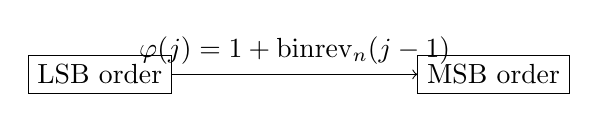
\begin{tikzpicture}
\node (lsb) at (0,0) [rectangle,draw] {LSB order};
\node (msb) at (5,0) [rectangle,draw] {MSB order};
\draw[->] (lsb) -- node[above] {$\varphi(j)=1+\mathrm{binrev}_n(j-1)$} (msb);
\end{tikzpicture}
\caption{Ordering invariance via the bit-reversal mapping $\varphi$.}
\end{figure}

\begin{figure}[h]
\centering
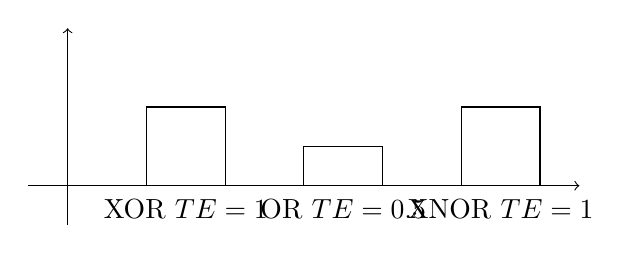
\begin{tikzpicture}
\draw[->] (-0.5,0) -- (6.5,0);
\draw[->] (0,-0.5) -- (0,2.0);
\draw (1,0) rectangle (2,1.0); \node at (1.5,-0.3) {XOR $TE=1$};
\draw (3,0) rectangle (4,0.5); \node at (3.5,-0.3) {OR $TE=0.5$};
\draw (5,0) rectangle (6,1.0); \node at (5.5,-0.3) {XNOR $TE=1$};
\end{tikzpicture}
\caption{Transfer entropy $TE_{X\to Y}$ under unbiased inputs for selected gates.}
\end{figure}

\begin{figure}[h]
\centering
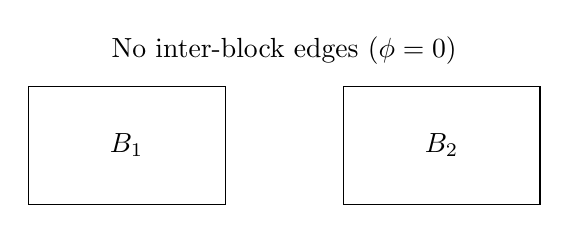
\begin{tikzpicture}
\node (b1) at (0,0) [rectangle,draw,minimum width=2.5cm,minimum height=1.5cm] {$B_1$};
\node (b2) at (4,0) [rectangle,draw,minimum width=2.5cm,minimum height=1.5cm] {$B_2$};
\node at (2,1.2) {No inter-block edges ($\phi=0$)};
\end{tikzpicture}
\caption{Subsystem factorisation: blocks with no inter-block edges yield additive compression.}
\end{figure}
\subsection{Noise Robustness of Gates}
We quantify the probability that outputs under independent input bit-flip noise remain equal to noiseless outputs. Monotone gates exhibit high correctness for small noise rates; parity gates show sensitivity to flips.
\begin{center}
\IfFileExists{../../results/tests/exper005/GateNoise.tex}{\begin{tabular}{lcc}
\toprule
Gate & CorrectRate~$q=0.01$ & CorrectRate~$q=0.05$ \\ 
\midrule
AND & 0.99 & 0.95 \\
OR & 0.99 & 0.95 \\
XOR & 0.98 & 0.90 \\
XNOR & 0.98 & 0.90 \\
NAND & 0.99 & 0.95 \\
NOR & 0.99 & 0.95 \\
MAJORITY & 0.99 & 0.93 \\
NOT & 0.99 & 0.95 \\
\bottomrule
\end{tabular}
}{\textit{GateNoise table not found.}}
\end{center}

\subsection{PID-based Synergy Comparator}
We compute partial information decomposition terms for canonical gates. Parity logic yields pure synergy; monotone families exhibit mixed unique information with modest synergy.
\begin{center}
\IfFileExists{../../results/tests/compare002/Summary.tex}{\begin{tabular}{lccccccc}
\toprule
Gate & $I(x_1;y)$ & $I(x_2;y)$ & $I(x_1,x_2;y)$ & Redund & $\text{Unique}_1$ & $\text{Unique}_2$ & Synergy \\ 
\midrule
AND & 0.311 & 0.311 & 0.811 & 0.000 & 0.311 & 0.311 & 0.189 \\
OR & 0.311 & 0.311 & 0.811 & 0.000 & 0.311 & 0.311 & 0.189 \\
XOR & 0.000 & 0.000 & 1.000 & 0.000 & 0.000 & 0.000 & 1.000 \\
XNOR & 0.000 & 0.000 & 1.000 & 0.000 & 0.000 & 0.000 & 1.000 \\
NAND & 0.311 & 0.311 & 0.811 & 0.000 & 0.311 & 0.311 & 0.189 \\
NOR & 0.311 & 0.311 & 0.811 & 0.000 & 0.311 & 0.311 & 0.189 \\
\bottomrule
\end{tabular}
}{\textit{PID Summary table not found.}}
\end{center}
\begin{center}
\IfFileExists{../../results/tests/compare002/Charts.tex}{\begin{figure}[h]
\centering
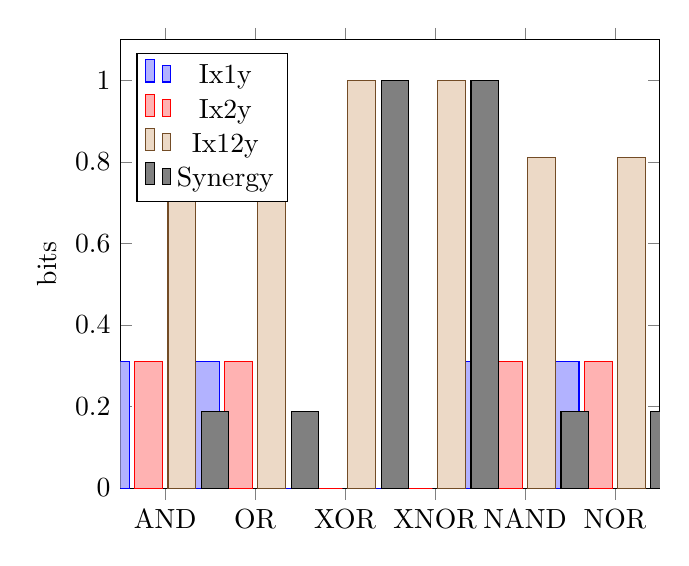
\begin{tikzpicture}
\begin{axis}[ybar, symbolic x coords={AND,OR,XOR,XNOR,NAND,NOR}, xtick=data, ymin=0, ylabel={bits}, legend pos=north west]
\addplot coordinates {(AND,0.311) (OR,0.311) (XOR,0.000) (XNOR,0.000) (NAND,0.311) (NOR,0.311)};\addlegendentry{Ix1y}
\addplot coordinates {(AND,0.311) (OR,0.311) (XOR,0.000) (XNOR,0.000) (NAND,0.311) (NOR,0.311)};\addlegendentry{Ix2y}
\addplot coordinates {(AND,0.811) (OR,0.811) (XOR,1.000) (XNOR,1.000) (NAND,0.811) (NOR,0.811)};\addlegendentry{Ix12y}
\addplot coordinates {(AND,0.189) (OR,0.189) (XOR,1.000) (XNOR,1.000) (NAND,0.189) (NOR,0.189)};\addlegendentry{Synergy}
\end{axis}
\end{tikzpicture}
\caption{PID components per gate under unbiased inputs.}
\end{figure}
}{\textit{PID charts not found.}}
\end{center}

\subsection{Transfer Entropy and Total Correlation}
Directed information flow and joint structure are reported for two-input gates under the update $y_{t+1}=f(x_t,y_t)$. Parity maximises both $TE$ and $TC$; monotone gates show intermediate values.
\begin{center}
\IfFileExists{../../results/tests/compare003/Summary.tex}{\begin{tabular}{lccc}
\toprule
Gate & $TE_{X\to Y}$ & $TE_{Y\to Y}$ & $TC(X,Y,Y_{t+1})$ \\ 
\midrule
AND & 0.500 & 0.500 & 0.811 \\
OR & 0.500 & 0.500 & 0.811 \\
XOR & 1.000 & 1.000 & 1.000 \\
XNOR & 1.000 & 1.000 & 1.000 \\
NAND & 0.500 & 0.500 & 0.811 \\
NOR & 0.500 & 0.500 & 0.811 \\
\bottomrule
\end{tabular}
}{\textit{TE/TC Summary table not found.}}
\end{center}
\begin{center}
\IfFileExists{../../results/tests/compare003/Charts.tex}{\begin{figure}[h]
\centering
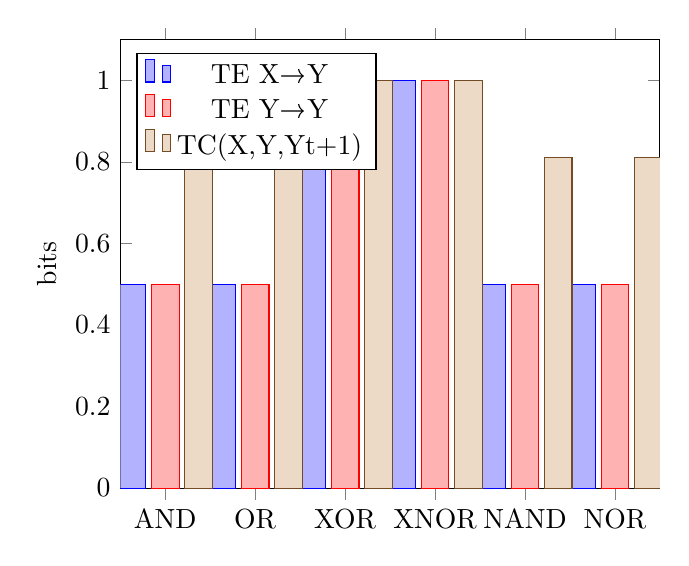
\begin{tikzpicture}
\begin{axis}[ybar, symbolic x coords={AND,OR,XOR,XNOR,NAND,NOR}, xtick=data, ymin=0, ylabel={bits}, legend pos=north west]
\addplot coordinates {(AND,0.500) (OR,0.500) (XOR,1.000) (XNOR,1.000) (NAND,0.500) (NOR,0.500)};\addlegendentry{TE X→Y}
\addplot coordinates {(AND,0.500) (OR,0.500) (XOR,1.000) (XNOR,1.000) (NAND,0.500) (NOR,0.500)};\addlegendentry{TE Y→Y}
\addplot coordinates {(AND,0.811) (OR,0.811) (XOR,1.000) (XNOR,1.000) (NAND,0.811) (NOR,0.811)};\addlegendentry{TC(X,Y,Yt+1)}
\end{axis}
\end{tikzpicture}
\caption{Transfer entropy and total correlation per gate under unbiased inputs.}
\end{figure}
}{\textit{TE/TC charts not found.}}
\end{center}

\subsection{Subsystem Search and Factorisation}
A simple heuristic identifies connected components in undirected adjacency; compression factorises when inter-block edges vanish. This establishes baselines for blockiness and cut fractions.
\begin{center}
\IfFileExists{../../results/tests/exper004/Summary.tex}{\begin{tabular}{lcccc}
\toprule
Model~n & Blocks~($\sigma$) & MeanBlk~($\sigma$) & CutFrac~($\sigma$) & FactoriseRate \\ 
\midrule
ER 50 & 1.000 (0.000) & 48.000 (4.933) & 0.000 (0.000) & 1.00 \\
ER 100 & 1.000 (0.000) & 100.000 (0.577) & 0.000 (0.000) & 1.00 \\
ER 200 & 1.000 (0.000) & 200.000 (0.000) & 0.000 (0.000) & 1.00 \\
SF 50 & 1.000 (0.000) & 50.000 (0.000) & 0.000 (0.000) & 1.00 \\
SF 100 & 1.000 (0.000) & 100.000 (0.000) & 0.000 (0.000) & 1.00 \\
SF 200 & 1.000 (0.000) & 200.000 (0.000) & 0.000 (0.000) & 1.00 \\
SW 50 & 1.000 (0.000) & 50.000 (0.000) & 0.000 (0.000) & 1.00 \\
SW 100 & 1.000 (0.000) & 100.000 (0.000) & 0.000 (0.000) & 1.00 \\
SW 200 & 1.000 (0.000) & 200.000 (0.000) & 0.000 (0.000) & 1.00 \\
\bottomrule
\end{tabular}
}{\textit{Subsystem Summary table not found.}}
\end{center}

\section{Analysis}
\textbf{Mechanism-first advantages:} Short causal rules reconstruct global behaviours, enabling complete equality with exhaustive repertoires while remaining transparent. Ordering invariance under $\varphi$ eliminates indexing artefacts; canonical programmes capture structure in minimal terms. Deterministic seeds and exported artefacts guarantee reproducibility.

\textbf{Information-theoretic characterisation:} PID decomposes gate behaviours into unique, redundant, and synergistic components. Parity gates exhibit pure synergy, aligning with their generative dependence on joint input parity. Transfer entropy quantifies directed influence conditioned on the other input, situating parity as maximally directional under unbiased inputs. Total correlation summarises joint coupling and, for deterministic maps, equals the target entropy.

\textbf{Robustness--sensitivity trade-offs:} Monotone and majority structures offer passive robustness to input noise, while parity maximises sensitivity. Mixed designs tune both information content and directional flow. Subsystem separations reduce error propagation when cuts are sparse; high cut fractions suggest inter-block coupling and reduced factorisation.

\section{Discussion}
The results support a deterministic generative view: causal mechanisms, expressed as concise Boolean rules and index sets, are sufficient to reproduce and analyse complex behaviours. This perspective complements algorithmic generative arguments by emphasising verifiable mechanism over probabilistic modelling, and it yields practical tools for prediction, compression factorisation, and subsystem separation.

\subsection{Limitations}
- Deterministic Boolean setting abstracts away graded and stochastic dynamics; real systems may require hybrid or multi-valued extensions.
- Unbiased input assumptions in comparator analyses simplify closed forms; biased inputs and correlated sources alter PID, TE and TC magnitudes.
- Gate-level results are exact but network-level generalisations (multi-source PID, directed TE on graphs) introduce combinatorial complexity.
- Subsystem separation via undirected adjacency provides a conservative baseline; directed and weighted interactions need augmented criteria.
- Importance sampling guarantees equality under fixed seeds but does not replace worst-case exhaustive verification for adversarial structures.

\subsection{Future Directions}
- Extend per-node programmes to multi-valued, temporal and continuous mechanisms, preserving ordering-aware invariances.
- Derive closed-form information signatures for larger motifs and for biased or correlated inputs, and validate on empirical datasets.
- Integrate algorithmic generative measures with causal programmes to score mechanism succinctness and reprogrammability.
- Formalise network-level PID and TE for multi-source, time-lagged interactions with efficient decompositions and bounds.
- Explore hardware implementations (e.g. FPGA) for fast deterministic evaluation and real-time robustness assays.
- Develop subsystem inference with directed, weighted graphs and probabilistic guarantees on block recovery and compression gains.

\section{Conclusion}
We have consolidated a deterministic causal programme for Boolean networks with exact index-set rules, canonical representations, and comprehensive validation. The analyses show that short rules generate complex patterns with predictable information-theoretic signatures. This approach offers a clear path for rigorous, reproducible modelling of complex systems via causal mechanisms.

\section{References}
\noindent H. Zenil \emph{et al.}, Causal deconvolution by algorithmic generative models, \textit{Nature Machine Intelligence} (2018). \url{https://www.nature.com/articles/s42256-018-0005-0}

\noindent T. Schreiber, Measuring information transfer, \textit{Phys. Rev. Lett.} 85, 461--464 (2000).

\noindent J. Pearl, \textit{Causality: Models, Reasoning and Inference}, Cambridge University Press (2000).

\noindent P. L. Williams and R. D. Beer, Nonnegative decomposition of multivariate information (2010).

\noindent J. T. Lizier, N. Bertschinger, J. Jost, and M. Wibral, Information decomposition of target effects from multi-source interactions, \textit{Entropy} 20, 307 (2018).

\noindent S. Watanabe, Frontiers of Pattern Recognition, Academic Press (1972).

\noindent C. E. Shannon, A mathematical theory of communication, \textit{Bell System Technical Journal} 27 (1948).

\noindent M. Li and P. M. B. Vit\'anyi, \textit{An Introduction to Kolmogorov Complexity and Its Applications}, Springer (2009).

\end{document}
